% Latex template: https://github.com/mqTeXUsers/Macquarie-University-Beamer-Theme

% Slide Masters:

% Title
% Text
% 2 column
% Full-image
% Bibliography
% Closing
 
\documentclass[aspectratio=169, 11pt]{beamer} % Aspect ratio
% https://tex.stackexchange.com/a/14339/5483 
% Possible values: 1610, 169, 149, 54, 43 and 32.
% 169 = 16:9

\PassOptionsToPackage{table}{xcolor}    %https://tex.stackexchange.com/a/5365/5483

\usetheme{macquarie}
\usepackage{multicol} % https://tex.stackexchange.com/a/396018/5483
\usepackage{xurl}
\usepackage[british]{babel}       % Set language
% \usepackage[utf8x]{inputenc}      % Set encoding
\usepackage{colortbl}
\mode<presentation>           % Set options
{
  \usetheme{default}          % Set theme
  \usecolortheme{default}         % Set colors
  \usefonttheme{default}          % Set font theme
  \setbeamertemplate{caption}[numbered] % Set caption to be numbered
}

% Uncomment this to have the outline at the beginning of each section highlighted.
%\AtBeginSection[]
%{
%  \begin{frame}{Outline}
%    \tableofcontents[currentsection]
%  \end{frame}
%}

\usepackage{graphicx}         % For including figures
\usepackage{booktabs}         % For table rules
\usepackage{hyperref}         % For cross-referencing


\usepackage{enumitem} % https://tex.stackexchange.com/a/2292/5483

%https://tex.stackexchange.com/a/371844/5483
\setbeamerfont{bibliography entry author}{size=\tiny}
\setbeamerfont{bibliography entry title}{size=\tiny}
\setbeamerfont{bibliography entry location}{size=\tiny}
\setbeamerfont{bibliography entry note}{size=\tiny}
\setbeamerfont{bibliography item}{size=\tiny}

%https://tex.stackexchange.com/q/333587/5483
%Uncomment to set (e.g.) an OSF URI for this presentation, license, etc.
\setbeamertemplate{footline}{\strut~CC-BY-4.0\hfill\insertframenumber~/~\inserttotalframenumber\strut~~~}

\usepackage{comment} % for commenting out multiple lines; uses \begin{comment} ... \end{comment}

\title{Transparency, reproducibility, and synthesis} % Presentation title
\author{A/Prof Shawn A Ross, Director of Data Science and eResearch}               % Presentation author
\institute{Office of the Deputy Vice-Chancellor (Research)}         % Author affiliation
\date{Monday 18 November 2019}                 % Today's date  
\begin{document}

% Title page
% This page includes the information defined earlier including title, author/s, affiliation/s and the date
% \begin{frame}[noframenumbering]

\begin{comment}

Abstract: 



Outline:

(1) Transparency, reproducibility, scalability today
-Reproducibility crisis
-Why? cognitive biases (ways we deceive ourselves, like confirmation bias or seeing patterns where there are none), professional pressures (journals like spectacular positive findings, not so interested in negative outcomes, despite the fact that falsification is important to the advancement of knowledge), poor research design (e.g., conflating inductive and deductive research), statistical errors
-'claimed research findings may often be simply accurate measures of the prevailing bias' \cite{Alberts2015-nq}
-Worse in social sciences and humanities: Sahlins, can you tell a paradigm from a fad? 'Paradigms change in the social sciences because,
their persuasiveness really being more political than empirical, they become commonplace universals. People get tired of them. They get bored.' \cite{Sahlins1999-is}
-Ideally, research is self-correcting, but emerging argument that active steps must be taken (new discipline of metascience)
-Response: improved research design (e.g., pre-commitment to approach, method, data collection, and analysis plan before starting research); transparency: make the process part of the product (e.g., data and analytical code)
-Should be done for its own sake, but also because otherwise archaeology will be sidelined in the emerging world of open scholarship (or, 'do you want to publish in Nature')
-Status quo so poor in archaeology that we don't even know if we have a problem (although indications are that we do...).
-Archaeology as a small data discipline has serious (but not unique) challenges.
-Problems will get worse, not better, if big data approaches like photogrametry, remote sensing, etc., come into common use without the basics (good / explicit design, FAIR data, analytical reproducibility) in place. 
-Archaeology tends to favour 'sharks and lasers'.
-Archaeology tends to neglect what is happening in neighbouring disciplines - striking difference going to the CAAs and going to RDA / CODATA - and it's the latter that feed into (e.g.) funder, publisher, and government policy
-Many of the same approaches that provide for transparency and reproducibility also contribute to scalability of research. Scalability arises largely from the ability to combine evidence ('data') from many sources, which requires that the data be technically and semantically interoperable. Such data is encouraged by FAIR principles and use of domain repositories (for example), automate routine processes (e.g., using the same code-based approaches that support analytical reproducibility), but good documentation of the project (explicit and sound research design) is also necessary. 
-None of these ideas are new in archaeology, many were raised in surprisingly contemporary language by early Processualists in the 1970s \cite{Hole1973-cy} - research design should drive your fieldwork, not methods, your approach should be explicitly stated, prioritise making your data compatible with that from other projects even at the expense of missed opportunities for marginal improvement.
-In this regard, our salvation lies in a 'back to basics' processualism, not naive empiricism or post-processual high theory.


(2) What does the future look like?
-Archaeology as a data science discipline more than a fieldwork discipline
-Archaeology as a discipline where registration of research design is routine (and all projects have a design: inductive / deductive / idiographic / nomothetic...research questions or hypotheses).
-Data structures, field processes, methods, etc. are fully documented and published
-Comprehensive, FAIR datasets are produced and deposited in domain repositories
-Analysis shifts from Excel and ARCGIS to code
-Processes / methods, data, and code are routinely reused
-We can have reasonable confidence in our results, self-correction can happen when we are wrong, and evidence / analysis can be combined from many projects to answer big questions.


\end{comment}


\maketitle

  
% \end{frame}

% Outline
% This page includes the outline (Table of content) of the presentation. All sections and subsections will appear in the outline by default.
\begin{frame}{The context of Research Data Management}
  \tableofcontents
\end{frame}

% The following is the most frequently used slide types in beamer
% The slide structure is as follows:
%
%\begin{frame}{<slide-title>}
% <content>
%\end{frame}


% Presentation providing context for the new data governance policies and procedures at Macquarie University

\section{The reproducibility crisis}

\begin{frame}{The `reproducibility crisis'}
  For nearly a decade the reproducibility crisis has featured in the scientific literature \cite{Jasny2011-bw, Baker2016-cf, Munafo2017-bj}. Low reproducibility rates have emerged from large-scale studies:
    \begin{itemize}[label=\textbullet]
        \item Results from only 39\% of psychology studies could be reproduced \cite{Open_Science_Collaboration2015-vf}.
        \item Even lower reproducibility rate in biomedical research \cite{Begley2012-xt,Prinz2011-za}.
    \end{itemize}
\end{frame}

\begin{frame}{Perceptions of the reproducibility crisis}
  \begin{figure}[H]
    \centering
        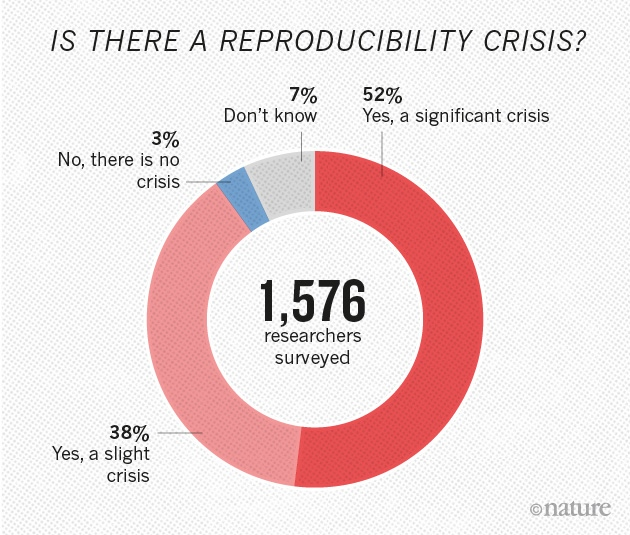
\includegraphics[height=.7\textheight]{figures/reproducibility-graphic-online1.jpeg}
        \caption{Is there a reproducibility crisis? \cite{Baker2016-cf}}
        \label{fig:Baker2016}
  \end{figure}
\end{frame}

\section{Causes of the crisis}

\begin{frame}{Data loss}
 \begin{figure}[H]
    \centering
        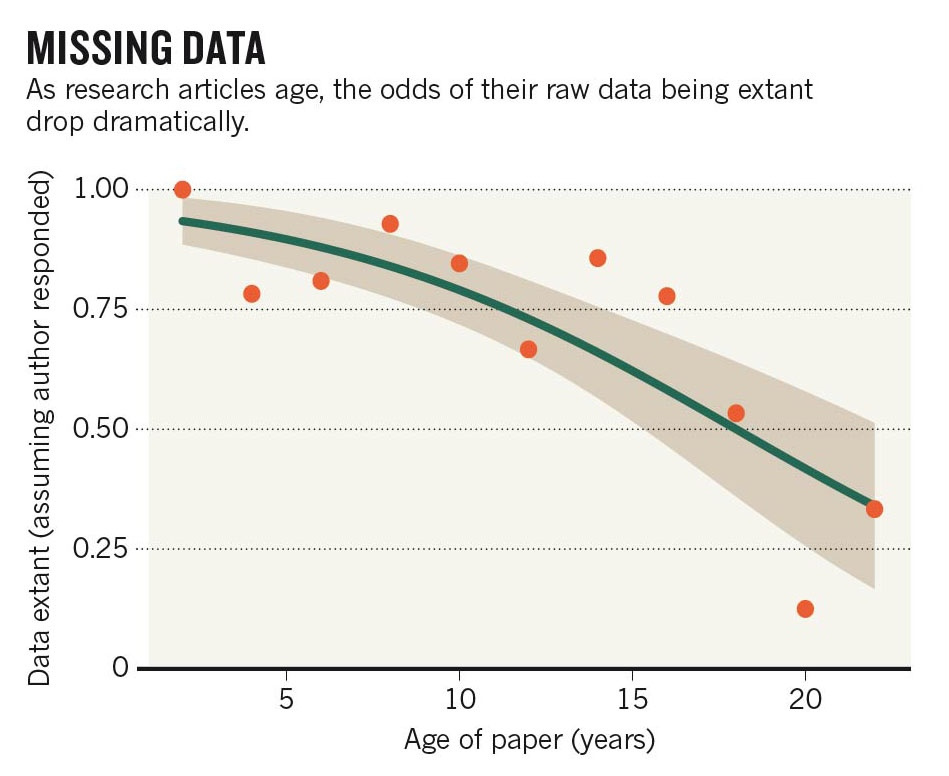
\includegraphics[height=.75\textheight]{figures/Missing-Data.png}
        \caption{\cite{Vines2014-zr}}
        \label{fig:vines2014}
 \end{figure}
\end{frame}

\begin{frame}{Big picture causes}
    \begin{itemize}[label=\textbullet]
        \item Opaque data and analysis practices. \cite{Marwick2017-bz}
        \item Professional pressures and cognitive biases unmitigated by good research design \cite{Muthukrishna2019-kt}
    \end{itemize}
    `Claimed research findings may often be simply accurate measures of the prevailing bias'. \cite{Alberts2015-nq} \par
\end{frame}

\section{Archaeology and the Open Scholarship movement}

\begin{frame}{Self-correction}
Ideally, research is self-correcting, but active steps must be taken.
    \begin{itemize}[label=\textbullet]
        \item Improved research design (e.g., pre-commitment to approach, method, data collection, and analysis plan before starting research).
        \item Transparency around evidence and analysis (e.g., provide comprehensive datasets and analytical code).
    \end{itemize}
\end{frame}

\begin{frame}{Better data and analytical practice}
  Manifestos, statements, and guidelines:
    \begin{itemize}[label=\textbullet]
        \item OECD Priniples and Guidelines for Access to Research Data \cite{Oecd2007-vi}.
        \item Findable, Accessible, Interoperable, and Reusable (FAIR) data \cite{Wilkinson2016-mr, Go-fair2017-vs}.
        \item Transparency and Openness Promotion (TOP) guidelines \cite{Nosek2015-wm, Cos2019-mr}.
        \item Data transparency toolkit \cite{Perkel2018-rw}.
    \end{itemize}
\end{frame}

\begin{frame}{Open Scholarship challenges}
    \begin{itemize}[label=\textbullet]
        \item We do not even know how bad the reproducibility problem is.
        \item Archaeology shares `small data' challenges.
        \item In technology, preference for `sharks with laser beams' over difficult and painstaking data management. 
        \item Problems will get worse, not better, if bigger data approaches like photogrammetry, come into common use without the fundamentals of data practice in place.
        \item Archaeology tends to be provincial - compare CAA versus RDA / CODATA. 
    \end{itemize}
\end{frame}

\begin{frame}{`Small data' research}
 \begin{figure}[H]
    \centering
        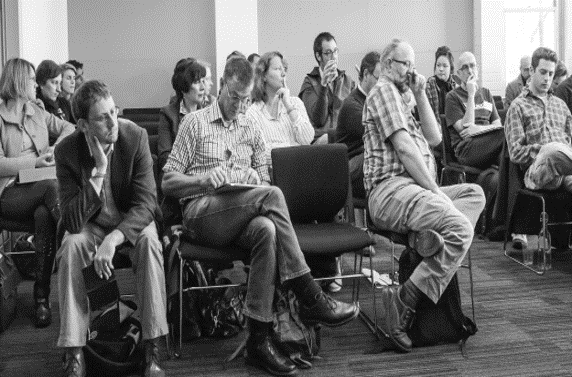
\includegraphics[height=.75\textheight]{figures/Archaeologists-standards.png}
        \caption{Archaeologists contemplate data standards (FAIMS Stocktaking, 2012)}
        \label{fig:figure7}
 \end{figure}
\end{frame}

\begin{frame}{Context: the challenge of `small data'}
    `Long tail' research: most field data is small data \cite{Borgman2015-rh}
    \begin{itemize}[label=\textbullet]
        \item Smaller scale; smaller communities; local control.
        \item Diverse questions, approaches, and methods.
        \item Heterogeneous data; variety of content, structure.
        \item Data and infrastructure emerge from fieldwork. 
        \item Relative lack of standards.
        \item Limited infrastructure and funding.
        \item Challenges associated with big(ger) data from photogrammetry, SfM, video, geophysics, etc., will exacerbate these problems.
    \end{itemize}
\end{frame}

\begin{frame}{Data fundamentals...}
 \begin{figure}[H]
    \centering
        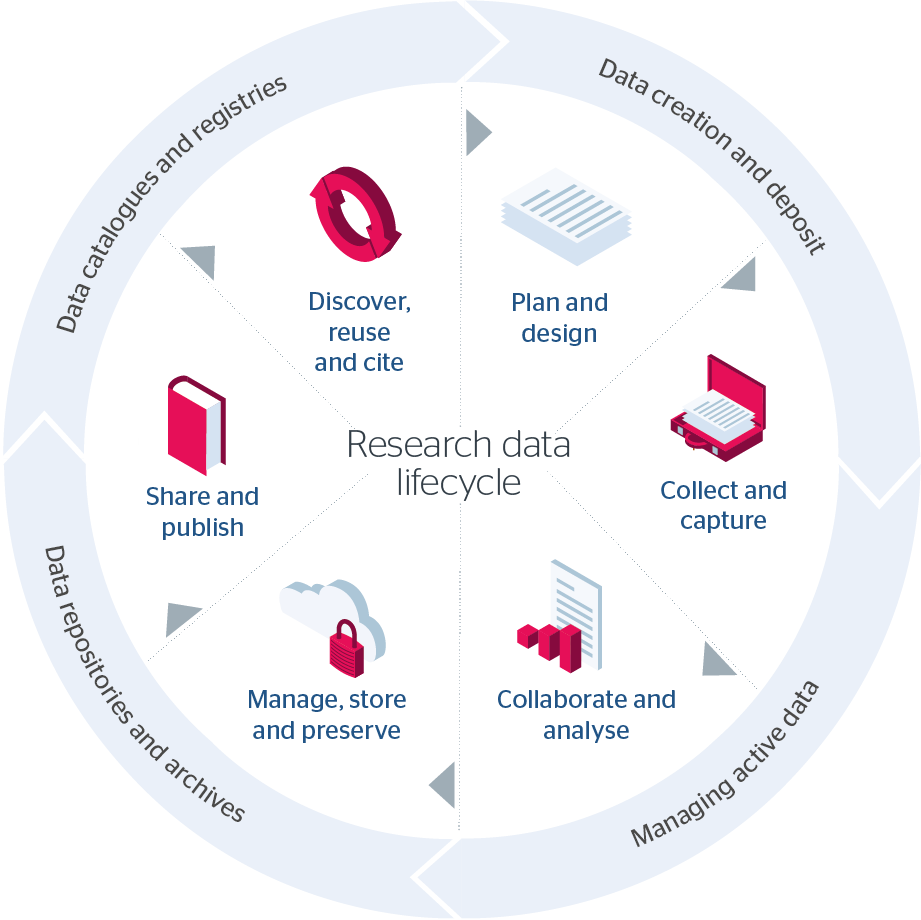
\includegraphics[height=.75\textheight]{figures/research-data-life-diagram.png}
        \caption{\cite{Jisc2018-gx} Image CC-BY-ND}
        \label{fig:figure9}
 \end{figure}
\end{frame}

\begin{frame}{...not `sharks with laser beams'}
 \begin{figure}[H]
    \centering
        
\includegraphics[height=.75\textheight]{figures/Sharks-Lasers.png}
        \label{fig:sharks}
 \end{figure}
\end{frame}

\begin{frame}{Open Scholarship resources}
    \begin{itemize}[label=\textbullet]
        \item History of re-evaluation of previous research.
        \item Many of the themes of Open Scholarship raised by early Processualists in the 1970s. \cite{Hole1973-cy} 
        \item Stable of leaders in Open Scholarship. \cite{Kansa2010-qx, Kintigh2006-wa, Marwick2017-bz}
    \end{itemize}
\end{frame}

\section{Change is coming}

\begin{frame}{Journal transparency mandates}
  Good practice should be done for its own sake, but also to avoid being sidelined as a discipline in the emerging world of Open Scholarship. \par
  Example mandates for transparency or reproducibility:
    \begin{itemize}[label=\textbullet]
        \item Nature: Transparency Upgrade \cite{Nature2017-lq}.
        \item Nature: FAIR data in Earth science \cite{Nature2019-ng}.
        \item Copernicus: FAIR data in atmospheric sciences \cite{Van_Edig2018-bu}.
        \item TOP Guidelines signatories include publishers representing 1000+ journals, as well as professional organisations and major private foundations  \cite{Cos2019-mr}.
    \end{itemize}
\end{frame}

% https://tex.stackexchange.com/a/2292/5483
% https://ctan.org/pkg/enumitem?lang=en

\begin{frame}{Level 2 TOP Guidelines for authors (excerpt)}
  
    \begin{enumerate}[label=\arabic*.]
        \setcounter{enumi}{1}
        % This increments the enumerate counter by 1.
        
        \item Authors using original data must:
        \begin{enumerate}[label=\alph*.]
            \item make the data available at a trusted digital repository [...]
            \item include all variables, treatment conditions, and observations described in the manuscript.
            \item provide a full account of the procedures used to collect, preprocess, clean, or generate the data.
            \item provide program code, scripts, codebooks, and other documentation sufficient to precisely reproduce all published results.
            \item provide research materials and description of procedures necessary to conduct an independent replication of the research.
        \end{enumerate}
    \end{enumerate}
    \cite{Osf2014-pf}
\end{frame}

\begin{frame}{TOP Guidelines: publisher adoption}
  \begin{figure}[H]
    \centering
        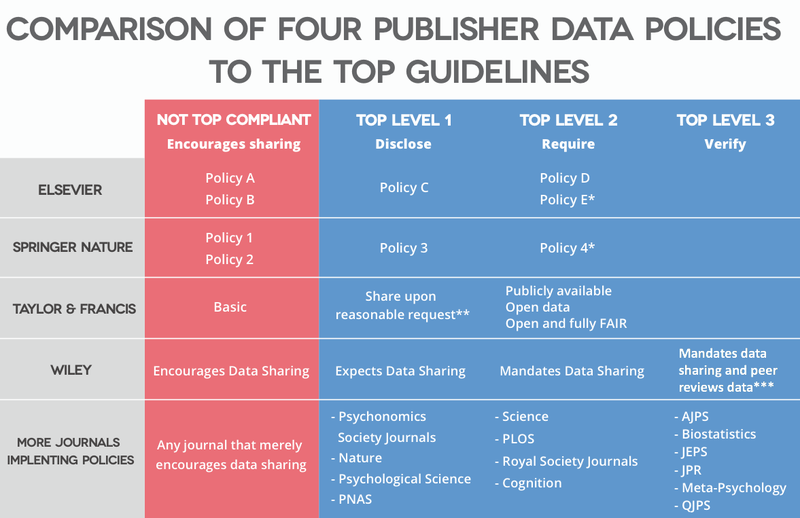
\includegraphics[height=.7\textheight]{figures/TOP-landscape.png}
        \caption{The Landscape of Open Data Policies \cite{Mellor2018-bf}}
        \label{fig:figure2}
  \end{figure}
\end{frame}

\begin{frame}{TOP Guidelines: funder endorsement}
  Private funders have endorsed via the Open Funders Research Group:
    \begin{itemize}[label=\textbullet]
        \item Alfred P. Sloan Foundation
        \item American Heart Association
        \item Bill and Melinda Gates Foundation
        \item Howard Hughes medical Institute
        \item John Templeton Foundation
        \item Laura and John Arnold Foundation
        \item Open Society Foundations
        \item Robert Wood Johnson Foundation
        \item Wellcome Trust
        \item and six more \cite{Ofrg2019-pq}
    \end{itemize}
\end{frame}

\begin{frame}{Other Funder data policies}
  \begin{figure}[H]
    \centering
        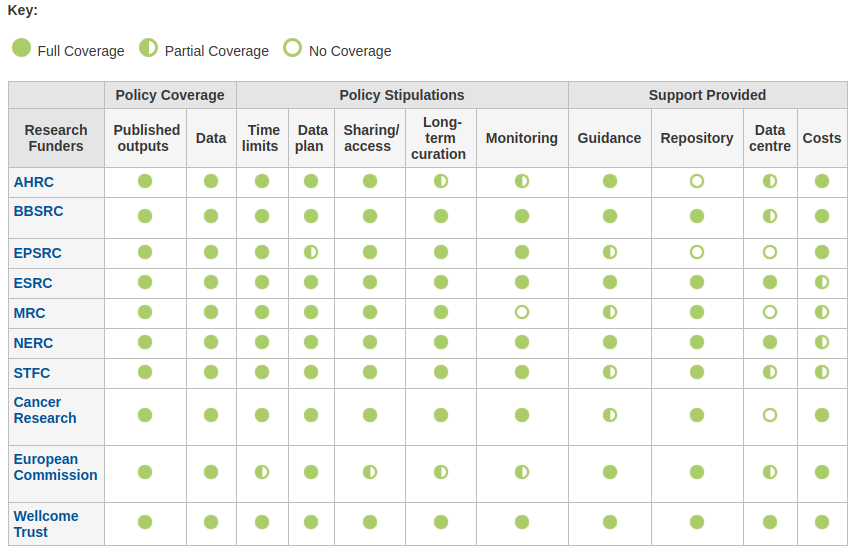
\includegraphics[height=.7\textheight]{figures/DCC-Funders.png}
        \caption{Overview of funders' data policies \cite{Dcc2019-jn}}
        \label{fig:Dcc2018}
  \end{figure}
\end{frame}

\begin{frame}{Not just the natural sciences}
  Changes are coming to HASS disciplines:
    \begin{itemize}[label=\textbullet]
        \item American Journal of Political Science requires (and tests) data and code \cite{Jacoby2017-lw, Ajps2015-ex}.
        \item All European Academies (allea) E-Humanities working group \cite{Allea2019-wy} has issued an Open Consultation on `Sustainable and FAIR Data Sharing in the Humanities' \cite{Allea2019-aw}.
        \item Allea seeks to address the imperatives of the `Open Science agenda' across Humanities and Social Sciences, and `facilitate the adoption of Open Science across the Humanities'.
        \item Research Data Alliance (RDA) has an 'Ambassador for the Humanities' and is examining how RDA standards and outputs can apply to humanities disciplines \cite{Rda2019-wc}.
    \end{itemize}
\end{frame}

\begin{frame}{Australia: Data sharing in the NHMRC Statement}
    The NHMRC `strongly encourages' data sharing in the National Statement on Ethical Conduct in Human Research and their Open Access Policy. \cite{Nhmrc2018-sj, Nhmrc2018-vn} \par
    National Statement 3.1.50 \par
    In the absence of justifiable ethical reasons (such as respect for cultural ownership or unmanageable risks to the privacy of research participants) and to promote access to the benefits of research, researchers should collect and store data or information generated by research projects in such a way that they can be used in future research projects. Where a researcher believes there are valid reasons for not making data or information accessible, this must be justified.
\end{frame}

\section{Beyond compliance: scaling research}

\begin{frame}{Large-scale research}
    The same approaches that facilitate transparency and reproducibility support the kind of scalable and synthetic research that can address archaeological `grand challenges'. \cite{Kintigh2014-ub}
        \begin{itemize}[label=\textbullet]
            \item Paper data capture and manual digitisation and cleaning don't scale.
            \item Collaboration based on email and desktop software doesn't scale.
    \end{itemize}
    
\end{frame}

\begin{frame}{Scalable approaches to data and analysis}
  \begin{figure}[H]
    \centering
        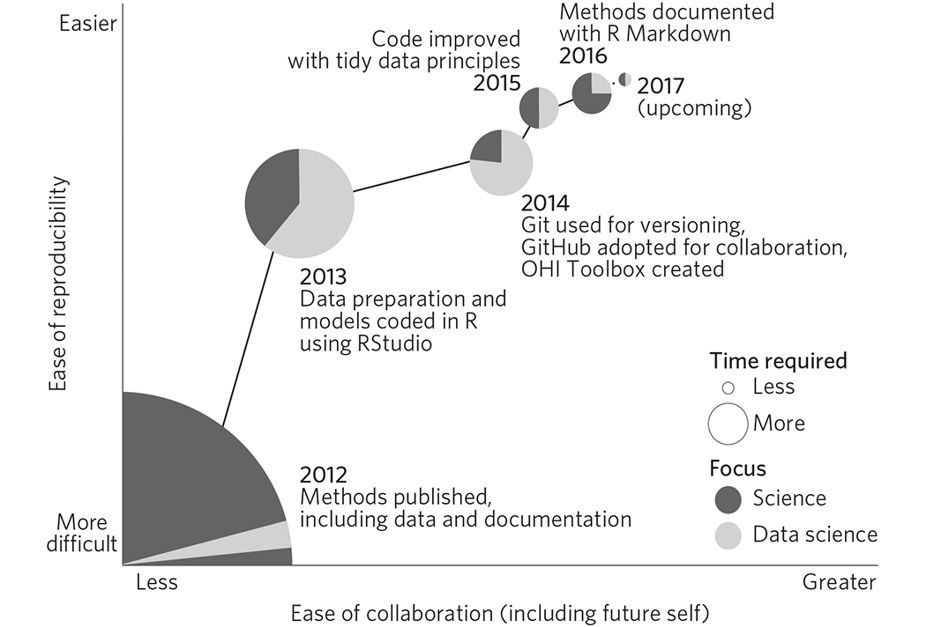
\includegraphics[height=.7\textheight]{figures/Ocean-Health-Index.jpg}
        \caption{Better science in less time, illustrated by the Ocean Health Index project. \cite{Stewart_Lowndes2017-lj}}
        \label{fig:stewart_lowndes}
  \end{figure}
\end{frame}

\section{What does the future look like?}

\begin{frame}{What does the future look like?}
    \begin{itemize}[label=\textbullet]
        \item Archaeology as a data science discipline more than a fieldwork discipline.
        \item Archaeology as a discipline where registration of research design is routine (and all projects have a design: inductive / deductive / idiographic / nomothetic...research questions or hypotheses).
        \item Data structures, field processes, methods, etc. are fully documented and published.
        \item Comprehensive, FAIR datasets are produced and deposited in domain repositories. 
        \item Analysis shifts to code.
        \item Processes / methods, data, and code are routinely reused. 
        \item We can have reasonable confidence in our results, self-correction happens when we are wrong, and evidence / analysis can be combined from many projects to answer big questions.
    \end{itemize}
\end{frame}


\begin{frame}{Thank you!}

PDF and source code for this presentation is available at: 
\texttt{https://github.com/saross/TRS-Archaeology/releases/tag/v1.0}

This work is licensed under a Creative Commons Attribution 4.0 International License.

\end{frame}

% \bibliographystyle{apalike}

% Adding the option 'allowframebreaks' allows the contents of the slide to be expanded in more than one slide.
% The "1" comes from the outer theme"

\section{References}

\begin{multicols}{2}[]
\bibliography{references}
\bibliographystyle{apalike}
\end{multicols}


% \begin{frame}[allowframebreaks]{References}
  
%   \bibliography{references}
%   \bibliographystyle{apalike}
% \end{frame}

\end{document}